\documentclass[11pt]{article}
\usepackage{graphicx, float, amsmath}
\parindent=0in
\parskip=8pt
\begin{document}
\title{COMP 512 - Final Project Report}
\author{Luke Emery-Fertitta - Student ID: 260569374 \\ Jonathan Campbell - Student ID: 260481285}
\date{2015 December 4}
\maketitle

\section*{Architecture}

To distribute load over several servers, we created a middleware to communicate between the client and resource manager (RM) servers. The middleware will receive requests from the client and forward them to the appropriate resource manager server, each server being responsible for one resource. The middleware is also responsible for customer data, since it is assumed that the most popular transactions performed will include modification or reading of customer data.  \par

We use of transactions to manage data operations. We use strict two-phase locking via a transaction manager and lock manager located at the middleware node. The locality of these managers guarantees a minimum in the number of network hops in order to perform the transactional management overhead. Finally, the two-phase commit protocol is used for committing and aborting transactions. \par

\section*{Performance results}

\subsection*{Technique}

For both parts, we use testing clients that repeatedly submit two transaction types. One is a middle-ware only transaction containing three customer read operations and three write operations. The other uses all three resource managers, performing a read and a write at each one. Each experiment can have the number of clients and delay between transactions varied, allowing us to control transactions per second.

\subsection*{Results}

\begin{table}[H]
\centering
\caption{Performance of Single-Client Txn}
\begin{tabular}{c|c}
Type & Average Response Time(s) \\
\hline
Local MW & 0.0445 \\
Local RM & 0.1000 \\
Network MW & 0.0915 \\
Network RM & 0.1704 \\
\end{tabular}
\end{table}

\begin{figure}[H]
\centering
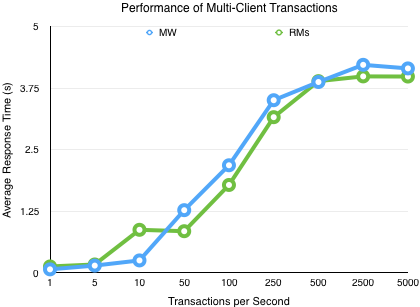
\includegraphics[scale=1]{plot.png}
\end{figure}

\subsection*{Analysis}

\textbf{Single-Client Observations:} \\
Network operations take roughly twice as long as local operations. RM transactions take roughly twice as long as their MW counterparts.\par

\textbf{Single-Client Analysis:} \\
Network latency explains the difference the local and network versions. We can use the numbers to estimate that time for each message. For example, 
\begin{align*}
\frac{0.0915 - 0.0445}{6}
\end{align*}
estimates the network time for each message. Additionally, the increased time for RM transactions is explained by the increased number of hops between nodes. \par

\textbf{Multi-Client Observation:}\\
Initially, RM-only transactions have a longer average response time than MW-only transactions. This swaps near 40 tps. After that, both increase at steady exponential rate (due to the logarithmic $x$-axis scale) with MW-only transactions being a constant amount above RM. At 500 transactions per second these amounts converge, followed by a slight increase in the response time on the part of the middleware. Both converge and plateau at 5000 transactions per second. \par

\textbf{Multi-Client Analysis:}\\
Between 1 and 40 tps, the RM transactions take longer due to the message transfer overhead. After this, the limiting factor is the bottlenecking due to lock conflicts, which continues to become more severe. At the time of this test, we used a 10 second deadlock detection, so our results are dominated by transactions that take 10 seconds. There may also be network congestion, contributing to the increase to a lesser degree. Finally, the plateau occurs due to the implementation of the Java client. The implementation is such that we are capped in the number of requests that can be actually sent, so despite the input parameters suggesting larger numbers of transactions per second, we are not actually increasing the number of requests per second.

\section*{Implementation of features}

\subsection*{Middleware}

The middleware system uses a new class that implements ResourceManager, and which maintains one WSClient for each resource manager server (flight, car, and room) for communication. Requests from the client are received through the Web Services interface. Each ResourceManager method involving flight, car, or room data will communicate with the appropriate Resource Manager using the relevant WSClient to invoke the smae method on that server.  \par

The middleware also maintains by itself all customer-related data in a hashtable. Methods that involve only customer data are processed directly at the middleware layer without any connection to an RM. Methods that involve both customer data and flight/car/room data, such as the reservation methods, or deleteCustomer, involve both processing by the middleware layer and communication with the appropriate resource managers.  \par

Since the middleware and server use the same class interface, the client can acquire the WSDL file from either. We chose to get it from the middleware so that the client doesn't need to know any information about the RM servers themselves.  \par

The middleware receives information about the RM servers (port and hostname) on server startup, through environment variables in the web.xml file.  \par

\subsection*{Lock Manager}

The lock manager is stored at the middleware server. It receives lock requests from the transaction manager, which specifies the lock type (read or write), the data item to lock, and the ID of the transaction requesting the lock. It uses this centralized model so that the resource managers themselves need know nothing about locking. This approach also simplifies the process of waiting on a lock, since the middleware will know not to accept anymore operations from the same transaction until the lock is received (or a deadlock occurs), instead of having to be told by a resource manager who is waiting that it should wait as well. \par

The lock manager uses the strict 2PL locking scheme. Operations that read a data item will request a shared lock on the item. More than one transaction can receive a shared lock for the same data item. Operations that write a data item will request an exclusive lock on the item, which will only be given if there are no shared locks on that item, except for its own. If the transaction does have a shared lock and requests an exclusive lock, the lock is converted to exclusive if possible. If other transactions already have a shared lock on that item, then the requesting transaction will wait until those are released. Transactions will release all their locks only at commit or abort time. \par

We chose to lock on entire resource managers. This was ultimately an oversimplification, and the issues with this assumption are discussed in greater depth in the ``Problems Encountered'' section of the report.\par

\subsection*{Transaction Manager}

The transaction manager is also contained entirely on the middleware server. Again, this design greatly simplifies the message passing requirements. Because the lock manager is local, the only message passing required after a request is received is the data access, which was already implemented in the first part of the project. Upon server initialization, a transaction manager is created. Then, we simply pass off the \texttt{start}, \texttt{abort}, and \texttt{commit} methods from the API directly to the transaction manager. \par

The \texttt{start} method initializes a transaction and provides the client with a transaction identifier to use with all other operations. This method atomically grabs the next available, unique transaction identifier integer, creates a \texttt{Transaction} object, and begins the TTL timer for the transaction. \par

When an operation is sent from the client to the middleware to be performed, the middleware will ask the transaction manager for the necessary locks and then perform the requested operation, forwarding it to a resource manager if appropriate. The transaction manager will also keep track of which data items are being locked, to be used later during the commit phase.

The \texttt{abort} method is available as an API call. Additionally, aborts will automatically be performed upon deadlocks, as a form of deadlock resolution, and TTL expirations, as a form of client timeout handling. The TTL expiration is checked by a \texttt{ScheduledExecutorService}, which is simply a scheduled, concurrent operation that ensures the transaction has been used within a specified time period. In this case, ``used'' refers to any read or write operation which is called with the transaction identifier.  \par

The \texttt{shutdown} method is an API call for a full-system, soft shutdown. If the client requests a shutdown, the transaction manager will deny any future start transaction requests and wait for all running transactions to complete. After this, each of the resource managers is sent a shutdown request and the middleware terminates. The resource managers will exit gracefully upon receiving the shutdown message from the middleware. \par

\subsection*{2PC}

The two-phase commit protocol was implemented on the transaction manager to coordinate commit and abort decisions in a distributed environment. The TM is responsible for all sending and receiving of vote requests and decisions. In brief, when a commit command is issued by the client, the transaction manager will send vote requests to all RMs (including the middleware, which handles the customer data) using a method call through Web Services. When a vote reply is received by an RM, a request is sent to the next in the list. If the RM fails to respond in a certain window of time (including if it crashes during the execution of the method call), the TM will consider the vote reply to be negative and begin aborting the transaction. The TM will also begin aborting the transaction as soon as it receives a negative response from any RM (e.g., if the first RM responds with a negative vote, then the transaction will be aborted without sending further vote requests to the remaining RMs).  \par

Once all vote requests have been received, and all are positive responses, the decision will be made to commit (otherwise, to abort). At this point, the TM will return from the commit() method to notify the client of its decision. Using a Future task, after the return of the method call, the TM will begin to inform the RMs (and middleware) of the decision to either commit or abort. (Only RMs that participated in the transaction to be committed will be notified of the decision.) The sending of vote decisions to each RM will block until the decision is successfully received by the RM, at which point the decision will begin to be sent to the next implicated RM. The blocking here is done to ensure that the decision is received by all RMs, in order to avoid an inconsistent state (i.e., to make sure that the decision communicated to the client was actually effectuated).  \par

Finally, once all resource managers have been informed, the TM will ask the lock manager to release all locks held by the transaction, and remove the transaction from its transaction list.  \par

\subsection*{Recovery}

In order to implement recovery, we keep keep logs at each node. These logs specify which stages of 2PC have been completed. The transaction manager logs the following steps for each transaction:
\begin{itemize}
\item commit/abort has started
\item no vote received
\item yes vote received
\item all votes received (prepared)
\item commit/abort decision sent
\item commit/abort complete
\end{itemize}
The resource managers log the following:
\begin{itemize}
\item vote request received
\item vote request sent (yes/no)
\item decision received
\item commit/abort complete
\end{itemize} 
Upon startup of a node, we look through the last log messages of each transaction. If we encounter a transaction that seems to be only partially completed, we will take whatever steps are necessary to finish the transaction as if the node had never been down.\par 

Each resource manager has an uncommited and committed data log stored on disk, so we use these logs to retrieve information in the case where we wish to finish commits upon recovery.\par

To persist information about transactions even if a crash occurs at the TM, transaction data is serialized to disk on any change of the data, and loaded back into main memory on server restart. This saving is necessary to persist the list of resource managers involved in any given transaction, so that if a crash interrupts the sending of vote requests to resource managers, the transaction manager will still know to which RMs a vote request should be sent.

\section*{Problems encountered}

One problem that was encountered that originated from the centralized model was the management of undo functions. Since the middleware contains the transaction manager, it is also responsible for informing the TM of the undo operations to perform in case of abort, before the actual operation takes place. Therefore, the middleware will need to know the reverse of each operation, even when it is only forwarding the operation to a resource manager. The undo operations are hardcoded in the middleware, so knowledge about each operation must reside at both middleware and RMs, which breaks the pattern of functional isolation. Further, some undo operations are more complex, in cases where an operation (like addFlight) can have different effects based on data state (it can add a completely new flight, or edit details of a current flight), leading to a necessity for state analysis on the middleware and communication with the RM to determine which action will be performed, in order to record the correct undo operation. \par

Concurrency was a concern due to the multithreaded request handling and asynchronus requirements of the transaction manager. We had to ensure that the transaction identifier was unique regardless of \texttt{start} execution order, and that once a shutdown request has been initiated, no client is able to start a new transaction. The former problem was solved with an \texttt{AtomicInteger} attribute, which allows for an atomic get and increment. The latter problem was solved by synchronizing the shutdown and start methods and adding an \texttt{isShutdown} attribute, such that once the shutdown has begun, threads will block at \texttt{start}, and after it finishes, transactions will fail to start. \par

For the third part of the project, a major problem was our decision to lock an entire resource manager, instead of individual objects. This did not cause difficulties in succeeding at the various tests of the second part, but was shown to be an oversimplification for the third part of the project. This locking constraint is too strict, and fails to allow for clients to perform certain operations that would never cause data consistency issues. In the future, fixing this would be the top priority for remedying our current application,\par

\section*{Testing}

\subsection*{Middleware}

Testing of the middleware was initially done manually, followed by a short series of JUnit tests. These tests act as an automated client, running a list of commands and verifying the results with assertions. This allows us to run detailed tests frequently, and without having to rely on human verification.  \par

\subsection*{Lock Manager}

To test the lock manager, we created a framework to easily specify transactions and their specific operations to be executed. A Transaction Simulation class (TxnSimul) receives as input a series of integers representing the operations that the transaction should execute, with each group of four integers specifying the transaction ID, data item, lock type (read or write), and the amount of seconds to sleep after executing the operation. With this latter argument, it is possible to interleave the operations of two different transactions. The TxnSimul objects once created are inserted into an array, and then a new thread is created for each, so that all run concurrently. We created several tests in this format to verify the integrity of the lock manager, including the following schedules, with reasoning for each:

\begin{itemize}
\item T1 reads A, T1 writes A, T1 commit (lock conversion)
\item T1 reads A, T2 reads B, T2 writes A, T1 writes B, T1 commit, T2 commit (deadlock detection)
\item T1 reads A, T2 reads A, T2 commit, T1 writes A, T1 commit (check that read lock can be acquired on object with read lock already, and unlocking of locks upon commit)
\item T1 reads A, T2 reads A, T1 writes A, T1 commit, T2 commit (check if shared lock blocks other's write)
\end{itemize}

Specific particularities of scheduling prevented by two-phase locking such as dirty reads, writes, unrepeatable reads, etc., were not tested here since it was assumed that the provided 2PL locking implementation was sound. \par

\subsection*{Transaction Manager}

With regards to testing of the transaction manager, sequences of commands were manually inputted into the client console with verification of results. Testing of undo operations was of particular focus, as well as concurrent modification situations (to verify correctness of locks).\par

\subsection*{2PC and Recovery}

In order to test 2PC and Recovery, we used crash points and console logging. The console logging confirmed that the commit protocol followed all of the steps properly. The crash points were useful for testing recovery. Through the client interface, we could specify the following locations for the nodes to crash:
\begin{itemize}
\item immediately (equivalent to a keyboard interrupt)
\item at the transaction manager, after sending some of the vote requests.
\item at the transaction manager, after receiving all of the vote replies.
\item at the transaction manager, after sending some of the commit/abort decisions.
\item at the transaction manager, after sending all of the commit/abort decisions.
\item at a resource manager, after receiving a vote requests.
\item at a resource manager, after sending a vote.
\item at a resource manager, after receiving a commit/abort decision.
\end{itemize}
For testing, we simply tried all of these crash points manually. Using the console logging and queries of information that should or should not be present, we were able to confirm the correctness of behavior for each case. We also added the ability to sent a nodes vote response. This allowed us to test scenarios where a node may have responded NO.\par

\end{document}
